\documentclass{article}

\usepackage[utf8]{inputenc}
\usepackage[french]{babel}

\usepackage{hyperref}
\usepackage{graphicx}
\graphicspath{ {./res/} }

\author{
    Valentin Jonquière,
    Mathilde Chollon,
    Denis Demirci,
    Iwen Jomaa,
    Jonathan Landry
}

\title{Rapport Préliminaire projet de programmation, Échecs en Java}

\begin{document}

\maketitle

\pagebreak

\tableofcontents

\pagebreak

\section{Contexte du sujet}
\subsection{Sujet choisi}
Nous avons choisi le sujet '\textit{les échecs}' car nous avons abordé ce jeu
plusieurs fois et dans différentes disciplines. Nous avions par exemple illustré un 
cours d'intelligence artificielle au semestre dernier avec celui-ci, mais 
également un cours d'algorithmie par le passé. Nous avons donc quelques connaissances 
utiles pour réaliser certains des besoins et qui nous permettent plus généralement de ne pas
découvrir entièrement le sujet.

\subsection{Langage de programmation choisi}
Avec ce sujet, nous avions 3 choix de langage possibles :
\begin{itemize}
    \item Le langage C
    \item Le Java
    \item Le Python
\end{itemize}
Même si nous avons dû faire un choix rapidement, nous avons d'abord développé les
avantages et inconvenants de chacun de ces langages. De plus, nous nous étions mis
d'accord sur quelques besoins essentiels auquel certains des langages ci-dessus 
n'aurait pas (ou difficilement) pu répondre.
Tout d'abord nous souhaitions pouvoir développer notre logiciel sous forme de modules
complémentaires, pour plusieurs raisons.
\begin{itemize}
    \item Nous avons convenu de baser les 8 semaines de code en se concentrant sur 
    des blocs de 2 semaines avec, pour chaque bloc, une liste de 2 ou 3 modules à développer.
    \item Isoler les bugs dans chaque module afin d'avoir moins de problèmes lors de la fusion
    des modules.
    \item Facilité de maintien. Avec 8 semaines de code, il est essentiel que nous possédions
    un logiciel organisé afin de ne pas avoir à `fouiller' dans le code écrit la première semaine
    lors de la finalisation du projet.
    \item Utilisation de la programmation objet. Même s'il n'y a pas d'extension de prévue,
    ce paradigme est le plus simple et adopté lors du développement d'un jeu.
\end{itemize}

\subsubsection{Langage C}
La première option qui nous était proposée été le langage C. Le projet contenant des besoins posant
des contraintes de performances (cf. besoin), ce langage a donc semblé être une bonne idée, car il est
de loin celui permettant d'obtenir un logiciel performant. Cependant, celui-ci ne proposant pas de 
possibilité de développement objet, nous aurions dû faire une grosse concession dès le choix du langage.
De plus, la gestion de la mémoire étant à la charge du développeur, nous aurions pu rester bloqué un temps
précieux sur un pointeur mal alloué. Cette gestion de la mémoire apporte également le problème des fuites
mémoire qui demandent, elle aussi, parfois beaucoup de travail pour être résolues.

\subsubsection{Python}
Nous pouvions également utiliser \textit{Python} pour réaliser ce projet. Cependant, le fait que ce langage
soit non typé a vite écarté ce choix. En effet, les types étant vérifiés directement à l'exécution, il est
beaucoup plus dangereux d'avoir une ligne non couverte par un test (il faut donc un coverage maximal). Il y
a donc le danger de laisser des erreurs de typages qui ne sont découverte uniquement lorsqu’une partie du code
est exécutée après la livraison du code.

\subsubsection{Java}
Nous avons donc fini par opter pour \textit{Java}. En effet, il permet tout comme \textit{Python} de faire
de la programmation objet, mais avec plus de rigueur. Étant conçu pour le développement objet, il y a moins
de chance de mélanger plusieurs paradigmes et de se retrouver avec un code mi-objet/mi-impératif. De plus,
le typage statique permet d'avoir une meilleure stabilité grâce à la détection des erreurs de types à la 
compilation et permet également d'avoir un code plus prévisible. Enfin, les plus projets réalisés en licence
et en master étant souvent des projets java, tous les membres du groupe connaissent ce langage ainsi que ses
outils et environnements de développement. Cela permettra de gagner du temps lors de la mise en place du projet. 
\section{Explication du sujet}

\section{Besoins visés}
\subsection{Quels besoins?}
Dans le sujet donné, il y avait une liste de 60 besoins.
Nous avons pris la décision ambitieuse de répondre à tous ces besoins. C'est un travail conséquent,
mais avec une équipe de 5 personnes, codant pendant huit semaines,
nous pensons que cet objectif est atteignable.

Nous avons tout de même classé ces besoins par ordre de priorité (voir \nameref{agenda}), afin de garantir
la jouabilité projet même si nous n'arrivons pas à tout implémenter à temps.
Nous voulons rendre un jeu cohérent et fonctionnel avec des modules entièrement
terminés (même s'il en manque) plutôt qu'un projet avec des règles manquantes,
une intelligence artificielle bâclée et une interface graphique peu fonctionnelle.

\subsection{Dépendances entre les besoins}
\subsubsection{Gestion des options}
La première dépendance que nous avons concerne la gestion des options.
\begin{figure}[h]
    \caption{Besoins concernant la gestion d'options}
    \centering
    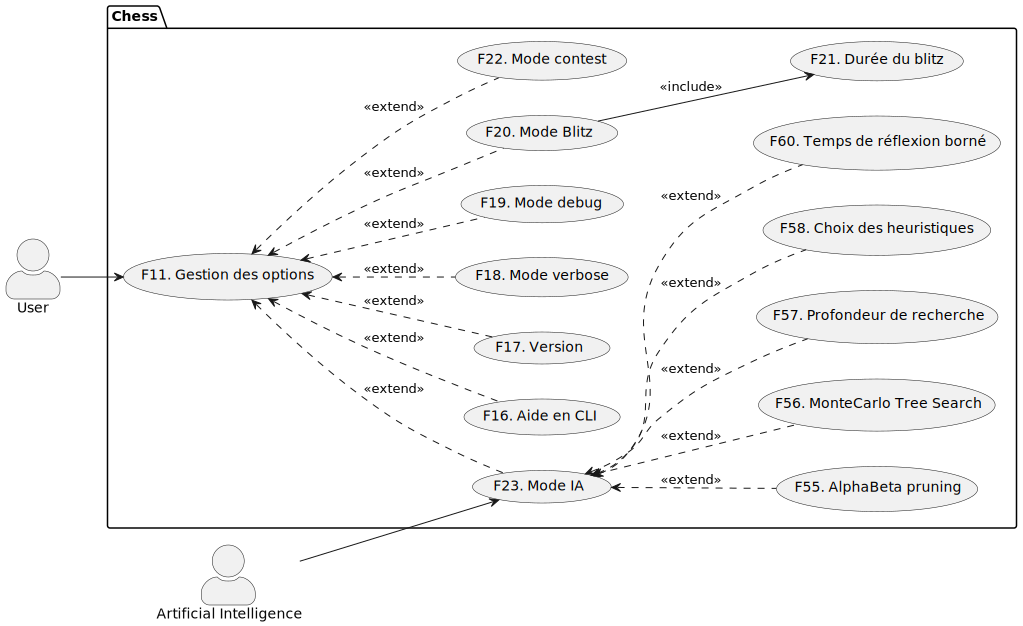
\includegraphics[width=\textwidth,height=\textheight,keepaspectratio]{needs_options}
\end{figure}

\subsubsection{Sauvegarde de l'historique}
La gestion de l'historique est un besoin indispensable pour notre jeu.
Beaucoup de besoins dépendent de cette fonctionnalité.
\begin{figure}[h]
    \caption{Besoins concernant la sauvegarde de l'historique}
    \centering
    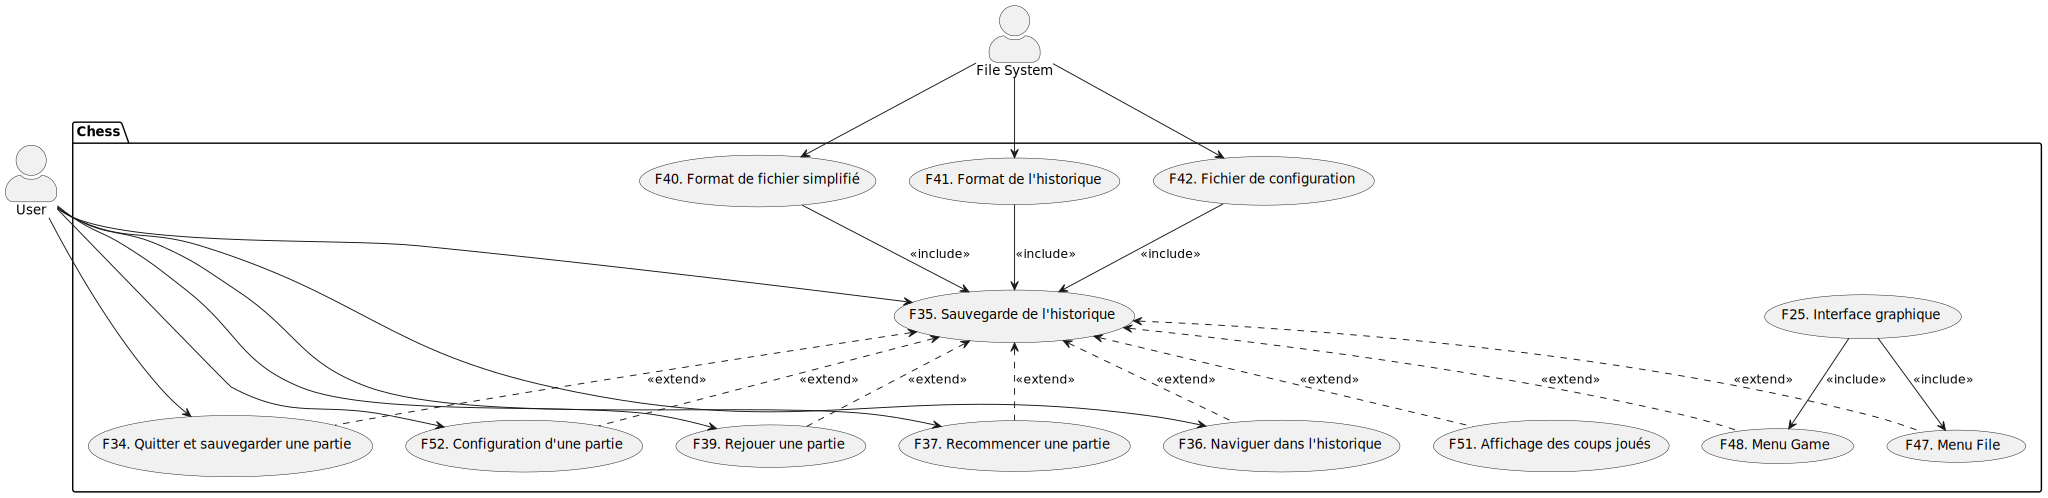
\includegraphics[width=\textwidth,height=\textheight,keepaspectratio]{needs_files}
\end{figure}

\subsubsection{Intelligence artificielle}
L'implémentation d'une intelligence artificielle est un autre besoin central du jeu. En effet, cela pourra
permettre à l'utilisateur de jouer contre une machine. Cela pourrait permettre également de donner des
indications sur les meilleurs coups à jouer pour le joueur.

\begin{figure}[h]
    \caption{Besoins concernant l'intelligence artificielle}
    \centering
    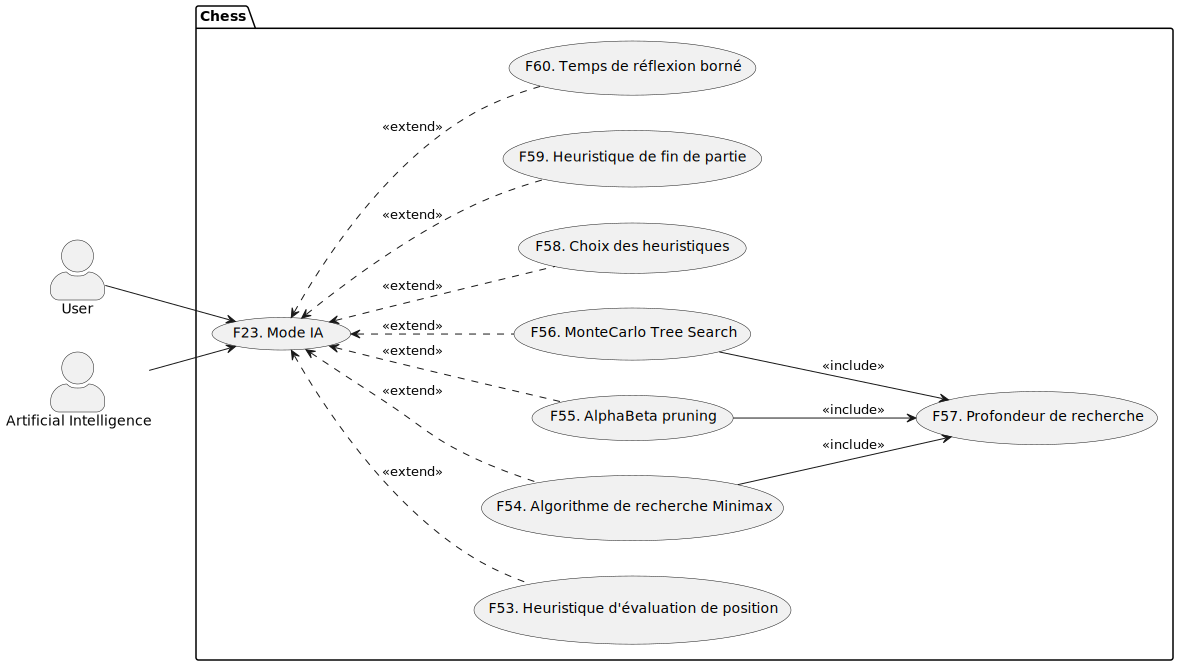
\includegraphics[width=\textwidth,height=\textheight,keepaspectratio]{needs_ai}
\end{figure}


Comme affiché Figure ???, nous pouvons voir que de nombreux besoins concernent l'intelligence artificielle.

\subsubsection{Interface graphique}
\begin{figure}[h]
    \caption{Besoins concernant l'interface graphique}
    \centering
    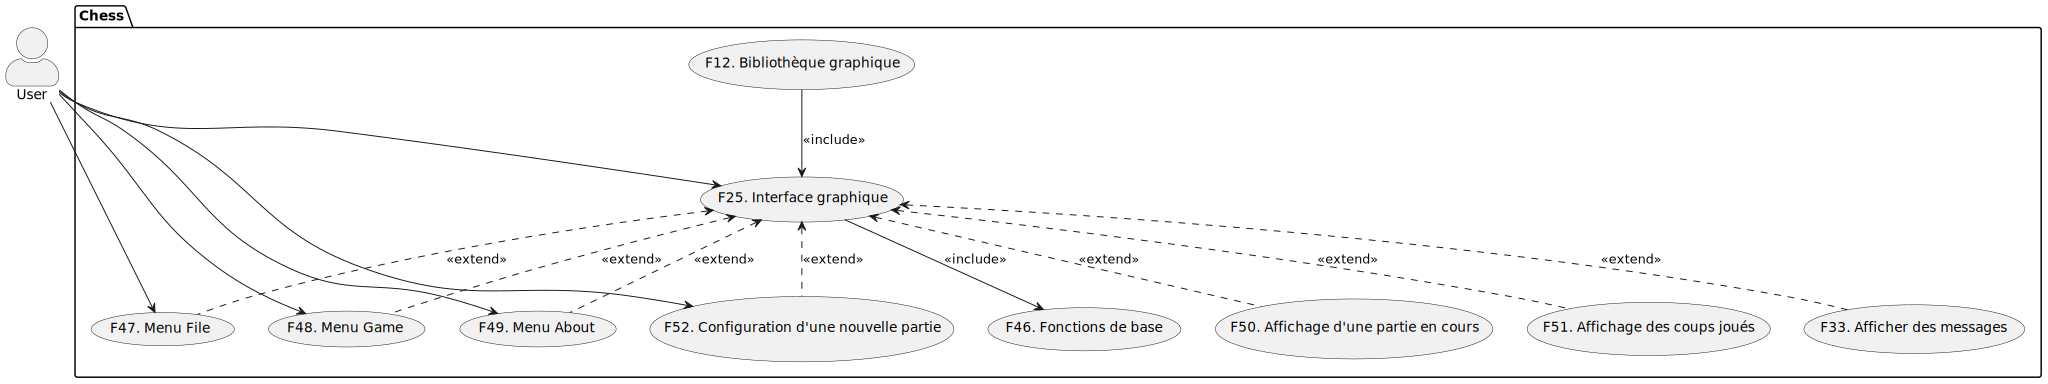
\includegraphics[width=\textwidth,height=\textheight,keepaspectratio]{needs_gui}
\end{figure}

\section{Agenda prévisionnel}
\label{agenda}

\section{Architecture visée pour le projet}

\section{Spécifications étendues}

\end{document}